\documentclass[11pt,a4paper]{article}
\usepackage[margin=22mm]{geometry}
\usepackage{amsmath,graphicx,booktabs,siunitx,hyperref}
\usepackage[T1]{fontenc}
\title{Complete pad histories with the optimized NAUSICAA CSA}
\date{\today}
\begin{document}
\maketitle
\section{Inputs and calculation}
The stored uncut ion counts provide a complete time sequence for each pad.
Missing sparse entries are filled with zero. Four files contain 8000 events each:
the same double-beta and electron samples at 2 mm pitch with 20 ms buckets and
4 mm pitch with 40 ms buckets. Each event starts with the CSA at its quiescent
operating point. Empty buckets and all large deposits are retained.

The circuit is the selected optimized 180 nm CSA: $C_f=3$ fF, external input
capacitance 1.25 pF, $M_f$ width 0.36 $\mu$m and length 400 $\mu$m, grounded
feedback gate, and $M_4$ gate at 0.6164 V. The output baseline is 0.884 V
and the fitted small-signal discharge time is 8.57 s.
Voltages are averaged over 5 ms centred at each frame boundary. The reported
frame signal is
\begin{equation}
 D_n=-[\Delta\overline V_n-\alpha\Delta\overline V_{n-1}],\qquad
 \alpha=\exp(-\Delta t/\tau),\qquad \Delta V=V-V_{\rm baseline}.
\end{equation}
Its low-charge gain is calibrated with the uniform-arrival SPICE packet.

Arrivals are uniform within each stored bucket. Each ion follows the on-axis,
constant-speed final approach used by the paper: a 0.5 mm square pad in a grounded
plane, 5 mm gap and speed 3 m/s. The pad weighting potential has unit pad and zero
surrounding-plane boundary conditions. This is the planar benchmark for the
finite-gap induced current. The input integral remains
$e[1-\phi_w(g)]$ per ion. No collection impulse or charge renormalization is added.

Julia first propagates every history using the calibrated small-signal packet
response and an exponential late tail. A minimum output of 0.2 V is used as a
diagnostic guard to select demanding cases. It is not a calibrated boundary of
linear operation. Three histories per input file are then simulated with the
full transistor circuit: the lowest predicted voltage, largest single bucket,
and the history closest to the guard.

\section{All-history linear screen}
\begin{table}[ht]
\centering\scriptsize
\begin{tabular}{lrrrrrr}\toprule
Sample & Events & Pads & Guard pads & Pads (\%) & Guard events & Events (\%)\\\midrule
2 mm, 20 ms, $0\nu\beta\beta$ & 8,000 & 2,268,244 & 0 & 0.0000 & 0 & 0.00 \\
2 mm, 20 ms, electrons & 8,000 & 2,807,207 & 0 & 0.0000 & 0 & 0.00 \\
4 mm, 40 ms, $0\nu\beta\beta$ & 8,000 & 703,623 & 335 & 0.0476 & 320 & 4.00 \\
4 mm, 40 ms, electrons & 8,000 & 874,715 & 246 & 0.0281 & 239 & 2.99 \\
\bottomrule\end{tabular}
\caption{Histories for which the linear output falls below the diagnostic 0.2 V
guard. These counts identify histories requiring nonlinear simulation.}
\end{table}
\begin{figure}[ht]\centering
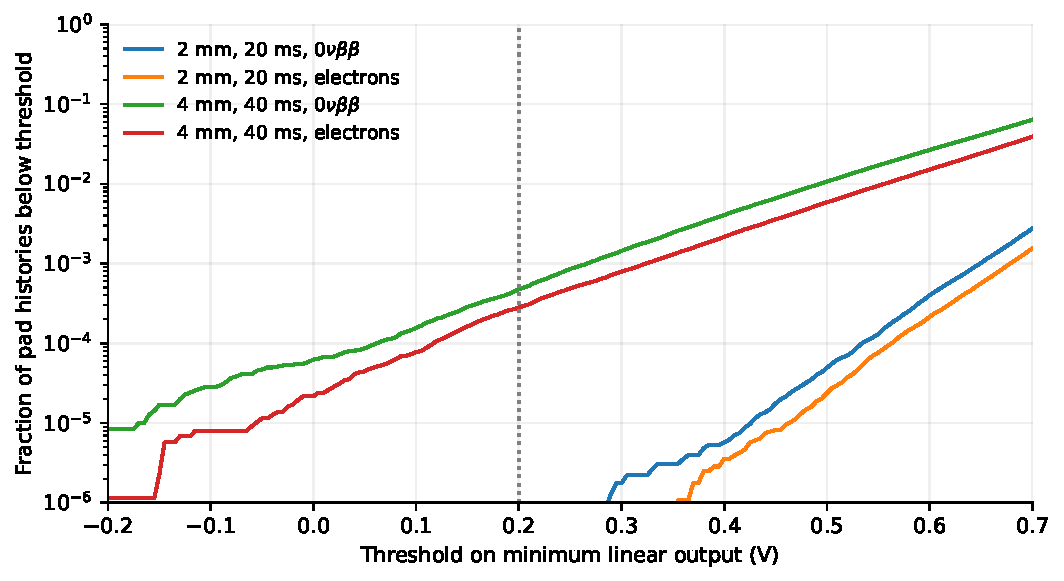
\includegraphics[width=.9\linewidth]{linear_screen.pdf}
\caption{Cumulative fraction of pad histories below a chosen minimum linear
output. Predictions below the supply range indicate failure of the linear approximation.}
\end{figure}

\section{Transistor-level histories}
Matched zero-input references and two time resolutions are used for all twelve
histories. Current transitions use 5 and 2.5 $\mu$s knot spacing; the solver maximum
steps are 0.5 and 0.25 ms. Each history includes 20 s of recovery after the stored
event interval. The maximum change of the frame signal under refinement,
normalized to its peak, is \num{1.793e-05}. The maximum relative input-charge error is
\num{2.934e-12}. The Julia accounting and zero-input checks pass (32 assertions),
as do the SPICE charge, refinement and voltage-bound checks (48 assertions).

\begin{table}[ht]\centering\scriptsize
\begin{tabular}{lrrrrr}\toprule
History & Event & $V_{\min}$ (V) & Recovery (s) & Positive ($e$) & Negative ($e$)\\\midrule
p2 $\beta\beta$, largest bucket & 7131 & 0.313 & 0.00 & 3.1 & -6.8 \\
p2 $\beta\beta$, near guard & 5407 & 0.282 & 0.00 & 8.0 & -0.6 \\
p2 $\beta\beta$, lowest linear voltage & 5407 & 0.282 & 0.00 & 8.0 & -0.6 \\
p2 e, largest bucket & 3390 & 0.421 & 0.00 & 0.0 & -0.7 \\
p2 e, near guard & 7641 & 0.278 & 0.00 & 8.7 & -0.6 \\
p2 e, lowest linear voltage & 7641 & 0.278 & 0.00 & 8.7 & -0.6 \\
p4 $\beta\beta$, largest bucket & 6831 & 0.202 & 0.00 & 65.4 & -1.2 \\
p4 $\beta\beta$, near guard & 3736 & 0.259 & 0.00 & 27.5 & -1.2 \\
p4 $\beta\beta$, lowest linear voltage & 3114 & 0.184 & 1.07 & 70.5 & -1.2 \\
p4 e, largest bucket & 2490 & 0.212 & 0.00 & 60.7 & -1.2 \\
p4 e, near guard & 6045 & 0.259 & 0.00 & 27.6 & -1.2 \\
p4 e, lowest linear voltage & 7756 & 0.196 & 0.21 & 67.3 & -1.2 \\
\bottomrule\end{tabular}
\caption{Actual output minima and recovery above the diagnostic guard, timed
from the last collection. The last two columns give extrema of the difference
between the nonlinear and linear frame estimates in empty buckets, starting one
full frame after the last collection. They use the low-charge gain to express
voltage in units of elementary charge.}
\end{table}

The extreme histories compress the output. A voltage minimum above the ground
rail therefore does not establish a linear response. In the selected cases the
output can remain below the guard after collection. Later positive residuals in
empty buckets remain smaller than one nominal quiescent ENC. The largest
negative residuals occur in the first evaluated empty bucket. Small residuals
in empty buckets do not establish that the gain for a new charge packet has
recovered while the output remains displaced.

Saturation flags should use a calibrated limit on CSA compression. ADC overflow
alone will not flag compressed signals that remain within its input range.
The event reconstruction can retain flagged deposits as high-charge locations;
its topology performance remains to be evaluated with these flags.

\begin{figure}[p]\centering
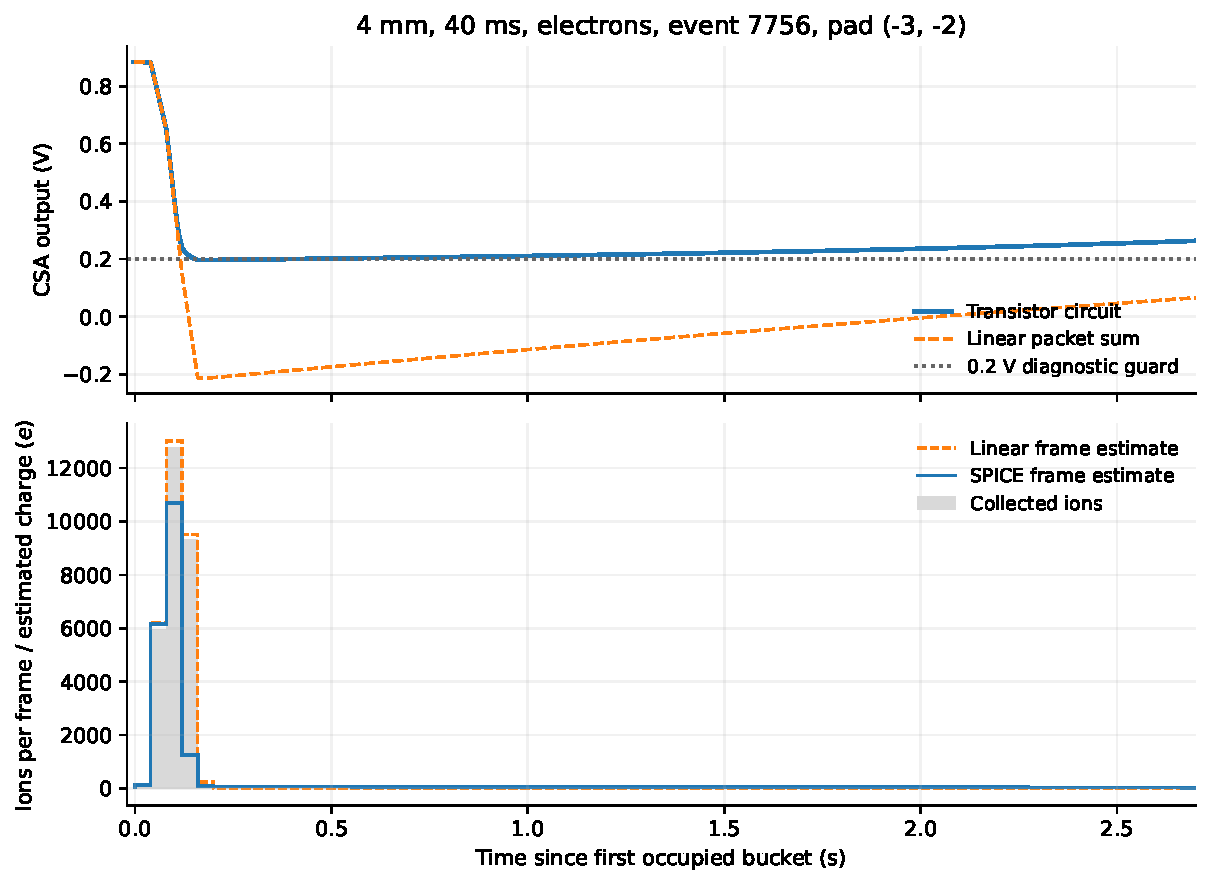
\includegraphics[width=\linewidth]{p4_electrons_worst_voltage.pdf}
\caption{A demanding electron pad history. The upper panel compares the full
transistor simulation with linear accumulation. The lower panel compares collected
counts and the charge inferred using the fixed low-charge gain.}
\end{figure}
\begin{figure}[p]\centering
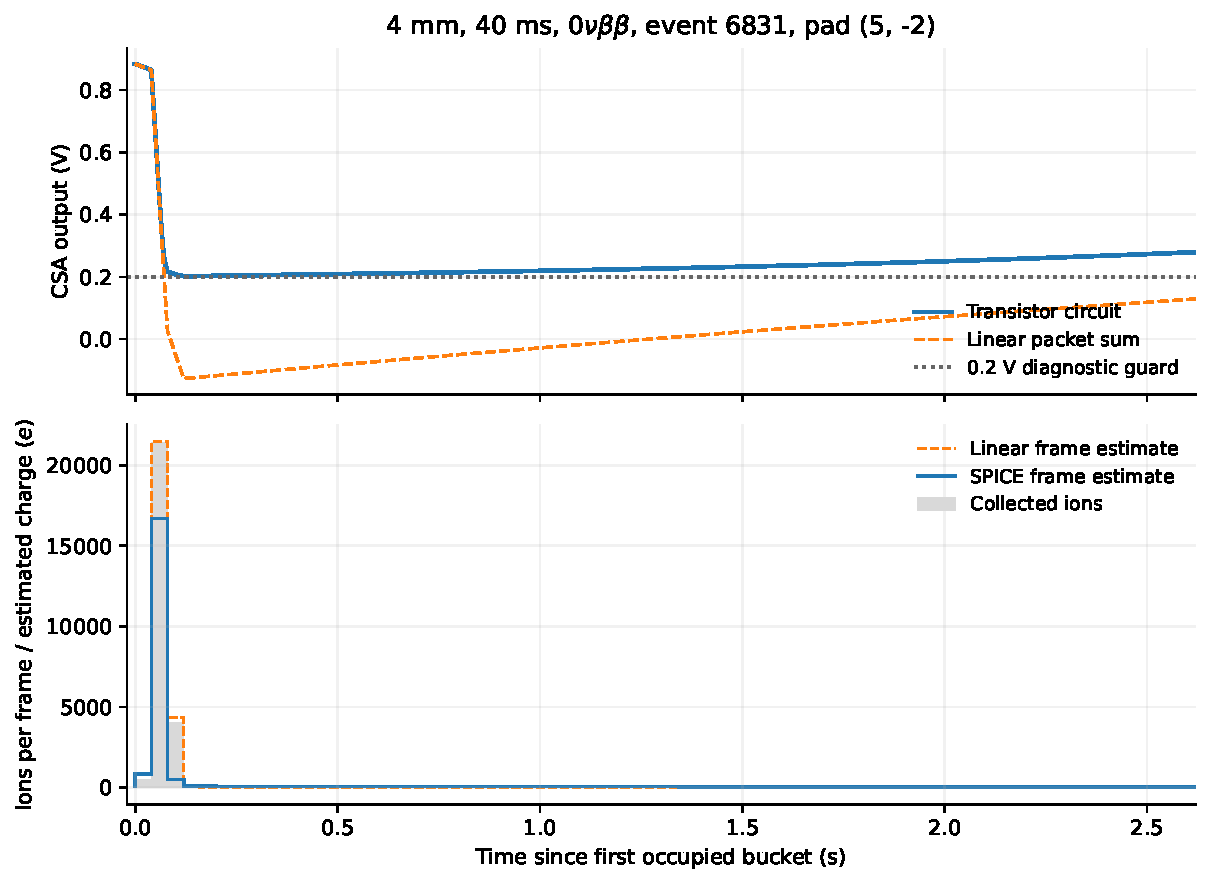
\includegraphics[width=\linewidth]{p4_bb0nu_largest_bucket.pdf}
\caption{The largest double-beta bucket at 4 mm pitch. Empty buckets retain the
circuit state and expose the recovery after the large deposit.}
\end{figure}

\section{ADC resolution}
\begin{table}[ht]\centering\small
\begin{tabular}{rrrrrr}\toprule
Frame (ms) & Span (V) & Bits & LSB ($\mu$V) & Quantization ENC ($e$) & RMS increase (\%)\\\midrule
20 & 1 & 10 & 977 & 10.82 & 1.548 \\
20 & 1 & 12 & 244 & 2.71 & 0.097 \\
20 & 1 & 13 & 122 & 1.35 & 0.024 \\
20 & 2 & 10 & 1953 & 21.64 & 6.056 \\
20 & 2 & 12 & 488 & 5.41 & 0.389 \\
20 & 2 & 13 & 244 & 2.71 & 0.097 \\
40 & 1 & 10 & 977 & 10.47 & 0.949 \\
40 & 1 & 12 & 244 & 2.62 & 0.060 \\
40 & 1 & 13 & 122 & 1.31 & 0.015 \\
40 & 2 & 10 & 1953 & 20.94 & 3.743 \\
40 & 2 & 12 & 488 & 5.24 & 0.238 \\
40 & 2 & 13 & 244 & 2.62 & 0.060 \\
\bottomrule\end{tabular}
\caption{Quantization contribution for independent uniform errors in the two
averaged voltage readings: $\sigma_{D,q}=\mathrm{LSB}\sqrt{(1+\alpha^2)/12}$.
The last column combines this contribution with the saved quiescent analogue noise.}
\end{table}
The selected SPICE histories fit within a 0--1 V input range. Twelve bits add
little noise even for a 2 V span. This resolution estimate assumes independent
uniform quantization errors on the averaged readings. It includes no reduction
from ADC oversampling and no additional ADC or buffer noise. The nominal ENC is
calculated at the quiescent operating point; noise at strongly displaced
operating points has not been evaluated in this study.

\section{Reproduction and provenance}
Physical propagation, PWL generation and numerical reduction are implemented in
\texttt{src/ion\_signal/pad\_history\_readout.jl} and
\texttt{src/ion\_signal/pad\_history\_spice.jl}. Python acquires LTspice output and
renders the saved HDF5 results. From the repository root, run
\begin{verbatim}
python scripts/run_pad_history_pipeline.py --simulator /path/to/LTspice
\end{verbatim}
Existing matching inputs and raw results are reused. Presentation alone is
\begin{verbatim}
python scripts/present_pad_histories.py
\end{verbatim}
The report source is generated without compiling the PDF. The numerical files
are in \texttt{results/ltspice/pad\_history\_readout/}. Configuration, code, source,
model, simulator and netlist hashes are stored with the results.

Input-file SHA256 identifiers:
\small
\noindent results/pixel\_charge\_1mm\_direct/bb0nu.h5\\{\ttfamily\scriptsize 4b2039511f4afb942bd845a074f2c62d064e4bb2a44e41e5cf5ba8ea06877a51}\par
\noindent results/pixel\_charge\_1mm\_direct/electrons.h5\\{\ttfamily\scriptsize b6388fdcdc1a9ebfab8dce1e02f325bb1e9b8048e4a4303ab2c737c1fe98e667}\par
\noindent results/pixel\_charge\_1mm\_4mm\_direct/bb0nu.h5\\{\ttfamily\scriptsize 9bb51f121de600b62f021fd560ef8a408cda3f137d72ce66f142cafa7a10267c}\par
\noindent results/pixel\_charge\_1mm\_4mm\_direct/electrons.h5\\{\ttfamily\scriptsize b6d04725bd693691e00c883642b4f2a8956cbd924467b8357d325879182acf90}\par
\end{document}
